%%% LaTeX Template originaly created by Karol Kozioł (mail@karol-koziol.net) and modified for ShareLaTeX use

\documentclass[a4paper,10pt]{article}

\usepackage[T1]{fontenc}
\usepackage[utf8]{inputenc}
\usepackage{graphicx}
\usepackage[dvipsnames]{xcolor}
\usepackage[british]{babel}
\usepackage[german=quotes]{csquotes}

%\renewcommand\familydefault{\sfdefault}
%\usepackage{tgheros}
%\usepackage[defaultmono]{droidmono}

\usepackage{amsmath,amssymb,amsthm,textcomp}
\usepackage{enumerate}
\usepackage{multicol}
\usepackage{tikz}

\usepackage{xcolor}

\usepackage{geometry}
\geometry{left=25mm,right=25mm,%
bindingoffset=0mm, top=20mm,bottom=20mm}
\usepackage{graphicx}
%\usepackage{subcaption}
%\usepackage{mwe}


\linespread{1.3}

\newcommand{\linia}{\rule{\linewidth}{0.5pt}}

% custom theorems if needed
\newtheoremstyle{mytheor}
    {1ex}{1ex}{\normalfont}{0pt}{\scshape}{.}{1ex}
    {{\thmname{#1 }}{\thmnumber{#2}}{\thmnote{ (#3)}}}

\theoremstyle{mytheor}
\newtheorem{defi}{Definition}

% my own titles
\makeatletter
\renewcommand{\maketitle}{
\begin{center}
\vspace{2ex}
{\huge \textsc{\@title}}
\vspace{1ex}
\\
\linia\\
\@author \hfill \@date
\vspace{4ex}
\end{center}
}
\makeatother
%%%

% custom footers and headers
\usepackage{fancyhdr}
\pagestyle{fancy}
\lhead{}
\chead{}
\rhead{}
%\lfoot{Assignment \textnumero{} 5}
\cfoot{}
\rfoot{Page \thepage}
\renewcommand{\headrulewidth}{0pt}
\renewcommand{\footrulewidth}{0pt}
%

% code listing settings
\usepackage{listings}
\lstset{
    language=Python,
    basicstyle=\ttfamily\small,
    aboveskip={1.0\baselineskip},
    belowskip={1.0\baselineskip},
    columns=fixed,
    extendedchars=true,
    breaklines=true,
    tabsize=4,
    prebreak=\raisebox{0ex}[0ex][0ex]{\ensuremath{\hookleftarrow}},
    frame=lines,
    showtabs=false,
    showspaces=false,
    showstringspaces=false,
    keywordstyle=\color[rgb]{0.627,0.126,0.941},
    commentstyle=\color[rgb]{0.133,0.545,0.133},
    stringstyle=\color[rgb]{01,0,0},
    numbers=left,
    numberstyle=\small,
    stepnumber=1,
    numbersep=10pt,
    captionpos=t,
    escapeinside={\%*}{*)}
}

% ref packages
\usepackage{nameref}
% folowing  must be in this order
\usepackage{varioref}
\usepackage{hyperref}
\usepackage{cleveref}

\setlength\parindent{0pt}

%%%----------%%%----------%%%----------%%%----------%%%

\begin{document}

\title{INF273 – Assignment 1}

\author{Lukas Schramm}

\date{\today}

\maketitle

\section*{Task 1a – Liner Shipping}
\subsection*{Description}
The task is to find a good representation of a solution of the \enquote{Liner shipping problem} as seen in figure \ref{fig:task1a}. There is a port in central Europe from which one ship will start to visit a couple of numbered Norwegian ports. There is the possibility to using small vessels which branch away from the main ship at one harbour, delivering goods to some harbours around the region until they get back into the harbour where they came from. The number of small vessels is not upperbounded.\footnote{It is of course formally upperbounded in the way that every vessel should serve at least one port, so there cannot exist more small vessels than ports to visit.}\medskip

\subsection*{Proposed solution}
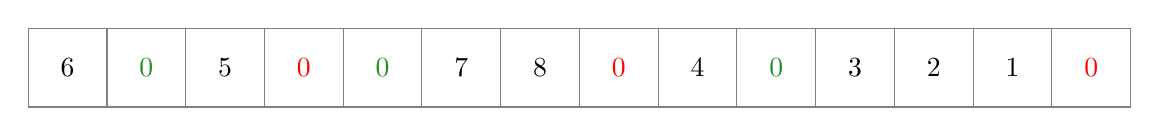
\begin{tikzpicture}
\draw[step=1cm,color=gray] (1,0) grid (15,1);
\node at (1.5,0.5) {6};
\node at (2.5,0.5) {\textcolor{ForestGreen}{0}};
\node at (3.5,0.5) {5};
\node at (4.5,0.5) {\textcolor{red}{0}};
\node at (5.5,0.5) {\textcolor{ForestGreen}{0}};
\node at (6.5,0.5) {7};
\node at (7.5,0.5) {8};
\node at (8.5,0.5) {\textcolor{red}{0}};
\node at (9.5,0.5) {4};
\node at (10.5,0.5) {\textcolor{ForestGreen}{0}};
\node at (11.5,0.5) {3};
\node at (12.5,0.5) {2};
\node at (13.5,0.5) {1};
\node at (14.5,0.5) {\textcolor{red}{0}};
\end{tikzpicture}\\
In my proposed solution, the order of numbers is the order of harbours which the main vessel is visiting. However, there are small subvessels which visit small harbours in behalf of the main vessel. Those are always sandwiched into in between two zeros. If there is a new subvessel which branches away from harbour $k$, then there is a zero after harbour the number $k$. Following that zero, the list contains the numbers of each harbour that subvessel is visiting. When it merges into the main vessel again, there is a second zero indicating that the main vessels journey continues again. This is easily possible since every subvessel returns to the place where it has started from.\\
If there is a known number of usable subvessels, then the solution has a fixed length. That length is the sum of the number of ports plus two times the number of subvessels. This is due to the fact that each harbour gets visited once and each subvessel has two zeros. In that fixed case, if a vessel is not used in any way, we just add the two times the number of unused vessels in zeros to the end of the list. This way it is constant.\\
However, if the number of those vessels is not fixed, we do not need any extra zeros in the end, but the list size shrinks and extends depending on adding or removing subvessels.\\
Conditions:
\begin{itemize}
\item There is an even number of zeros. In the example above, I visualised those with green and red colour, where the green onces (every odd one) start a vessel, while the red ones (the even onces) finish a vessel.
\item Each number (except for the zero) appears \underline{exactly} one time
\item Every subvessel is sandwiched in within two zeros.
\end{itemize}

\begin{figure}[h]
\centering
\includegraphics[width=0.5\textwidth]{task1a}
\caption{Illustration of task 1a \enquote{Liner shipping}}
\label{fig:task1a}
\end{figure}

\clearpage


\section*{Task 1b – Trucks and Drones}
\subsection*{Description}
The task is to find a good representation of a solution of the \enquote{Truck and drones problem} as seen in figure \ref{fig:task1b}. The task is an extension of the travelling salesperson problem (TSP). Like in TSP, there is a heap of customers to deliver goods to which needs a routing plan from a start point via all the other points back to the origin. The difference for that problem is that there are up to $n$ drones\footnote{$n=2$ in the INF273 course} sitting on the roof of the truck which can deliver one customers each while the truck continues to a different customer. Every drone which visits a customer starts to branch away at a certain point, while they merge again with the truck at the customer afterwards. They cannot return to the original branching point since the track already left that one to visit its next customer. It is not possible to have more than $n$ drones in use at the same time.\medskip

\subsection*{Proposed solution}
This one is a bit harder compared to 1a since we now have the problem that drones do not return to the original place where they come from. But here, we have a fixed size of two drones and every drone only serves one place and then returns to the truck which already moved.\\

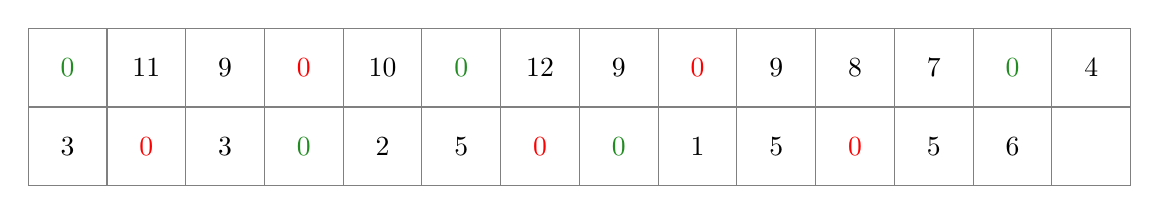
\begin{tikzpicture}
\draw[step=1cm,color=gray] (1,0) grid (15,2);
\node at (1.5,1.5) {\textcolor{ForestGreen}{0}};
\node at (2.5,1.5) {11};
\node at (3.5,1.5) {9};
\node at (4.5,1.5) {\textcolor{red}{0}};
\node at (5.5,1.5) {10};
\node at (6.5,1.5) {\textcolor{ForestGreen}{0}};
\node at (7.5,1.5) {12};
\node at (8.5,1.5) {9};
\node at (9.5,1.5) {\textcolor{red}{0}};
\node at (10.5,1.5) {9};
\node at (11.5,1.5) {8};
\node at (12.5,1.5) {7};
\node at (13.5,1.5) {\textcolor{ForestGreen}{0}};
\node at (14.5,1.5) {4};
\node at (1.5,0.5) {3};
\node at (2.5,0.5) {\textcolor{red}{0}};
\node at (3.5,0.5) {3};
\node at (4.5,0.5) {\textcolor{ForestGreen}{0}};
\node at (5.5,0.5) {2};
\node at (6.5,0.5) {5};
\node at (7.5,0.5) {\textcolor{red}{0}};
\node at (8.5,0.5) {\textcolor{ForestGreen}{0}};
\node at (9.5,0.5) {1};
\node at (10.5,0.5) {5};
\node at (11.5,0.5) {\textcolor{red}{0}};
\node at (12.5,0.5) {5};
\node at (13.5,0.5) {6};
\end{tikzpicture}\\
In that solution, there are also two zeros representing a drone which branches away from the main truck.\footnote{As in the task above, they are coloured in green and red to visualise their use.} Within these two zeros, there are always two numbers. The first number is the node where it branches away, while the second number it the node number where it merges with the truck again. If two drones start at the same node, they are also written directly each other, so a green zero follows directly on a red zero. The numbers in between describe the movement of the main truck. As in the last task, the number of zeros is even. Otherwise, it is unfortunately hard to describe more properties. Every non-zero number appears only once expect directly before a second zero, because those are the information where the drones return to. Since we have only two drones, it is not allowed to have more than one green zero after a red zero without a main truck number in between. The length of the solution is not fixed since we can send out our drones as often as we want.\\
It is a lot harder to validate that a solution is valid but it's still impossible. I am open for critics and nice alternative ideas.

\begin{figure}[h]
\centering
\includegraphics[width=0.5\textwidth]{task1b}
\caption{Illustration of task 1b \enquote{Truck and drones}}
\label{fig:task1b}
\end{figure}


\end{document}